\documentclass[14pt]{extarticle}
\usepackage{amsmath}
\usepackage{amssymb}
\usepackage{graphicx}
\graphicspath{ {../chap09/} }
\usepackage[top=1in, bottom=0.75in, left=0.75in, right=0.75in]{geometry}
\newcommand*{\Scale}[2][4]{\scalebox{#1}{\ensuremath{#2}}}%
\usepackage{hyperref}


\begin{document}

\section*{Math208 Discussion Outline for 11/03/2020}

\subsection{Homework and other due dates}
\begin{itemize}
\item Section 9.2 due 11/3
\item Section 9.4 - 9.5 due 11/6
\item Complete the Instruction Survey
\item In class assignment due 11/8 \\\\
\resizebox{12cm}{!}{
	{A photo that has meaning to you}
}
\end{itemize}

\subsection{Questions?}
\begin{itemize}
	\item HW 9.1 \#59 and Exam 2 \# 11
\end{itemize}

\subsection{Goals}
\subsubsection*{Section 9.2: Infinite Limits}
\begin{itemize}
	\item Identify and find infinite limits and vertical asymptotes
	\item Determine limits at infinity and horizontal asymptotes
\end{itemize}
\subsubsection*{Section 9.4: Infinite Limits}
\begin{itemize}
	\item Identify and find infinite limits and vertical asymptotes
	\item Determine limits at infinity and horizontal asymptotes
\end{itemize}
\subsubsection*{Section 9.5: Infinite Limits}
\begin{itemize}
	\item Identify and find infinite limits and vertical asymptotes
	\item Determine limits at infinity and horizontal asymptotes
\end{itemize}



\cleardoublepage



\subsection*{Section 9.2: Infinite Limits}
\subsubsection*{Some Graphs}
\begin{itemize}
	\item X-limits, \url{https://www.desmos.com/calculator/vshkxi2kdb}
\end{itemize}
%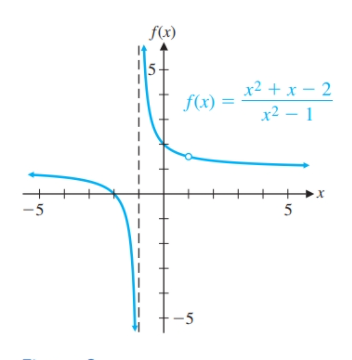
\includegraphics[width=0.3\linewidth]{9-2-1}
%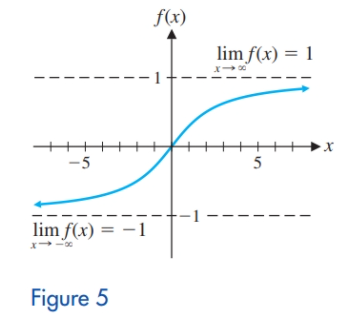
\includegraphics[width=0.3\linewidth]{9-2-4} 
\begin{center}
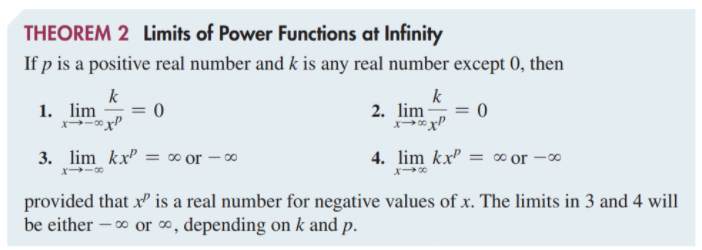
\includegraphics[width=0.9\linewidth]{9-2-5} \\
\end{center}


\begin{center}
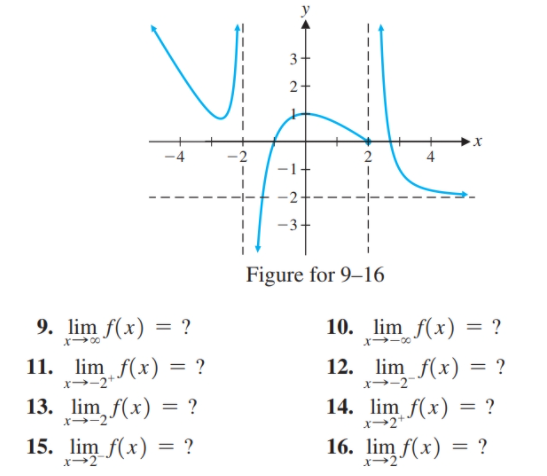
\includegraphics[width=0.7\linewidth]{9-2-8} \\
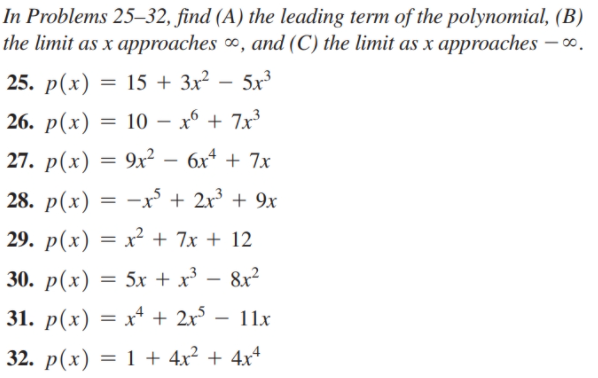
\includegraphics[width=0.7\linewidth]{9-2-9} \\
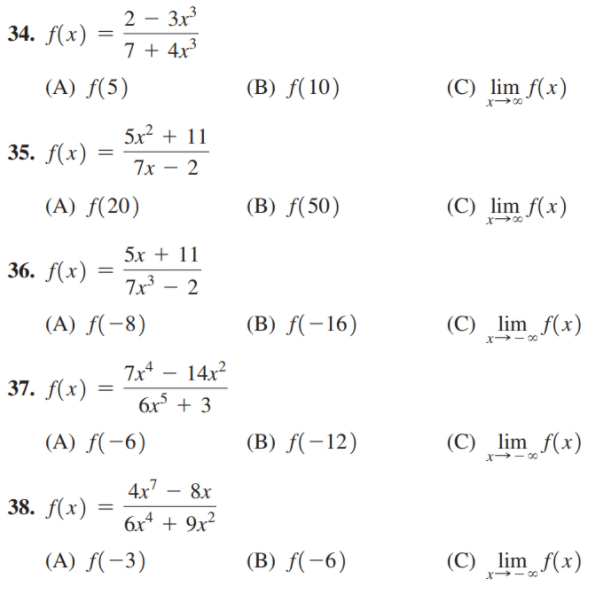
\includegraphics[width=0.7\linewidth]{9-2-10} \\
\end{center}

\cleardoublepage

\subsection*{Section 9.4: The Derivative}
\subsubsection*{Some Graphs}
\begin{itemize}
	\item Secant line to tangent line, \url{https://www.desmos.com/calculator/faudtsxdzy}
	\item Distance-velocity-accelerate, \url{https://www.desmos.com/calculator/jgxmedmm8n}
\end{itemize}
\subsubsection*{The Derivative}
\begin{itemize}
	\item Secant line is the line connecting any two points on the graph. This is usually expressed in point slope form where:
	\begin{align*}
		m = \frac{y_2-y_1}{x_2-x_1}
	\end{align*}
	then the secant line is:
	\begin{align*}
		y-y_1 = m(x-x_1)
	\end{align*}
\item Derivative
\begin{center}
	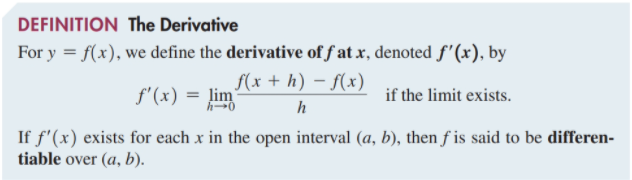
\includegraphics[width=0.95\linewidth]{9-4-1} \\
	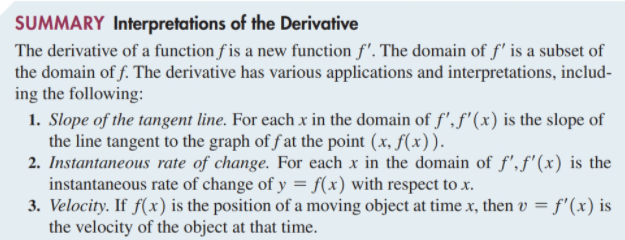
\includegraphics[width=0.95\linewidth]{9-4-2} \\
	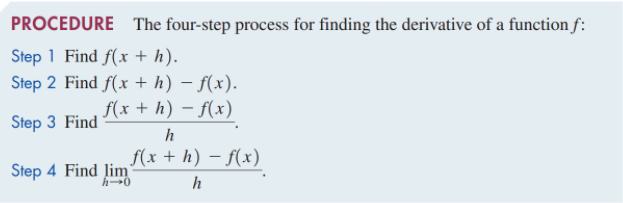
\includegraphics[width=0.95\linewidth]{9-4-3} \\
	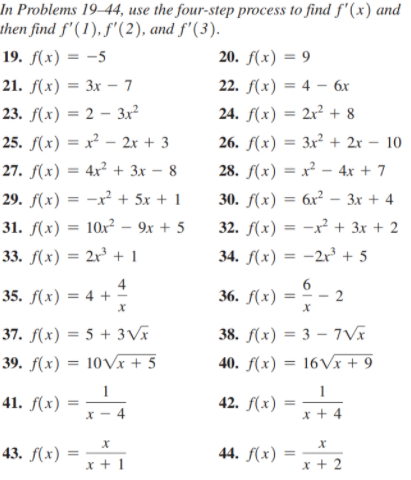
\includegraphics[width=0.8\linewidth]{9-4-4} \\
\end{center}
\end{itemize}

\subsection*{Section 9.5: Differentiation}
\begin{center}
	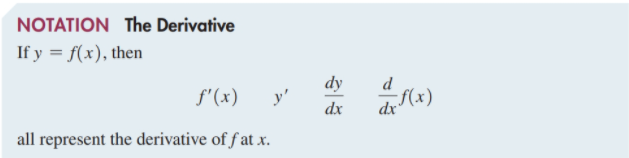
\includegraphics[width=0.8\linewidth]{9-5-1} \\
	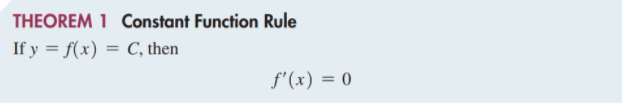
\includegraphics[width=0.8\linewidth]{9-5-2} \\
	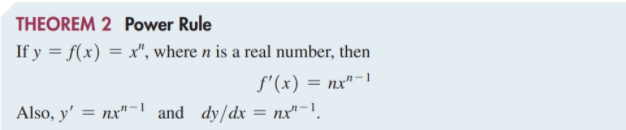
\includegraphics[width=0.8\linewidth]{9-5-3} \\
	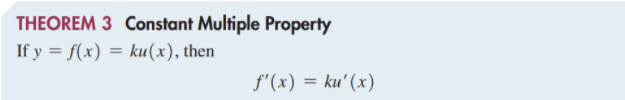
\includegraphics[width=0.8\linewidth]{9-5-4} \\
	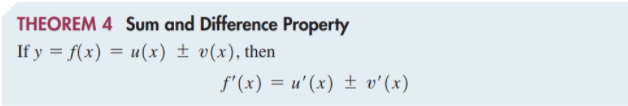
\includegraphics[width=0.8\linewidth]{9-5-5} \\
	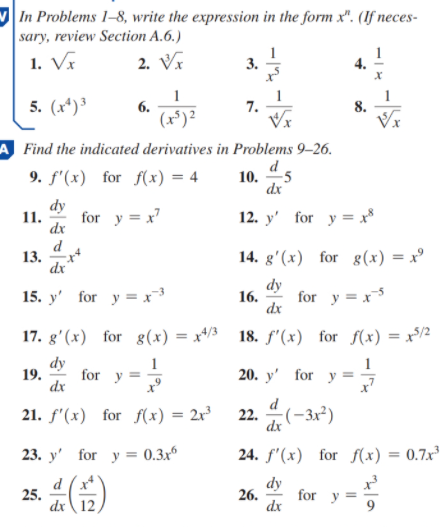
\includegraphics[width=0.7\linewidth]{9-5-6} \\
	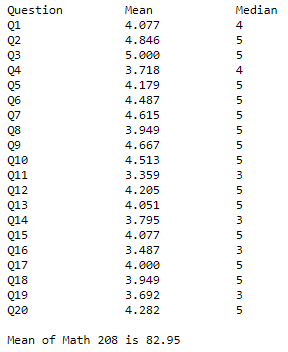
\includegraphics[width=0.4\linewidth]{exam2-results}
\end{center}






\end{document}
